\begin{document}

\maketitle

\section{Sissejuhatus}
\begin{frame}[fragile]
  \frametitle{Eelmine kord}
  Saame tuttavaks ja räägime strateegiast üldiselt
	\begin{itemize}
		\item Sissejuhatus: kes ma olen ja kuidas minu käest hinde saab
		\item IT seos äristrateegiaga, IT mõju ärile
		\item Süsteemidest ja tarkvara arhitektuurist
	\end{itemize}
\end{frame}

\begin{frame}[fragile]
  \frametitle{Täna kavas}
		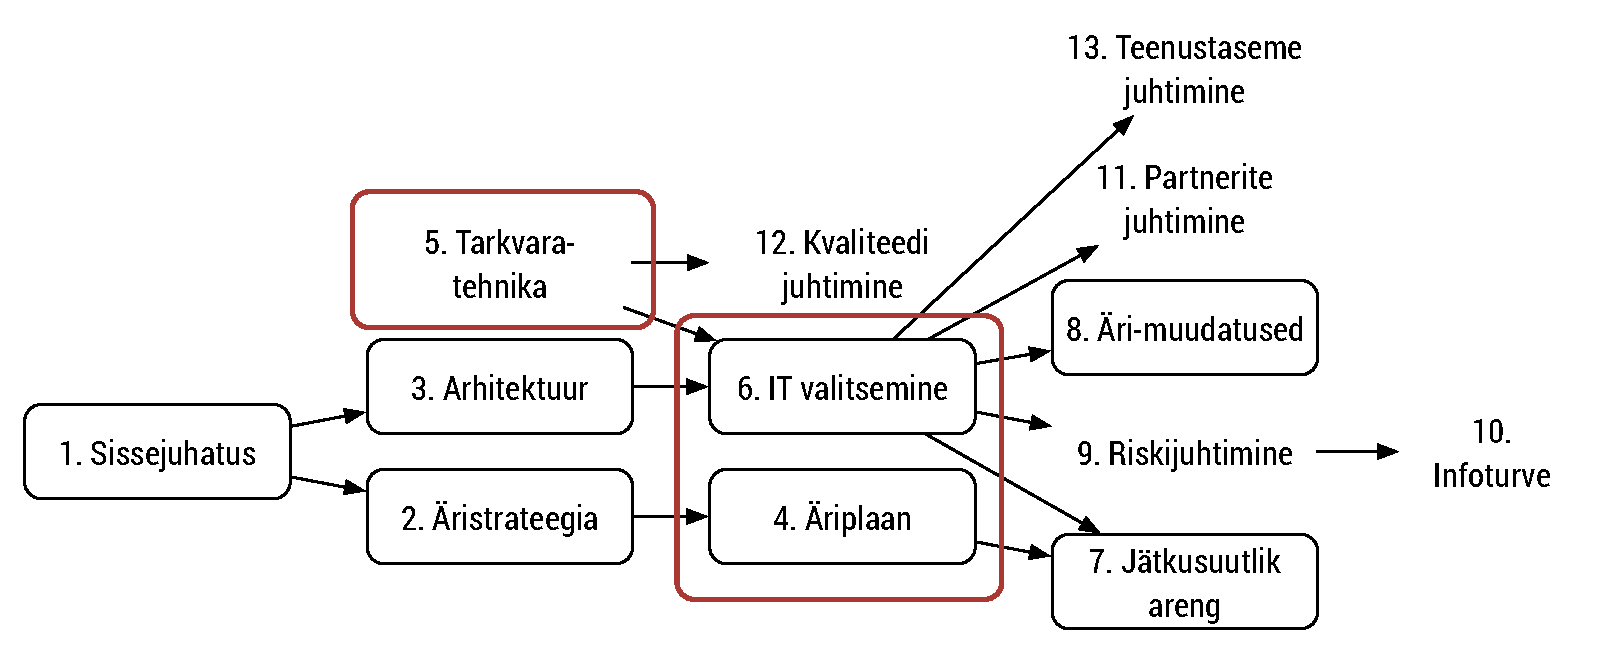
\includegraphics[width=\textwidth]{aine_struktuur_teine.pdf}
\end{frame}

\section{Äriplaani koostamine}
\begin{frame}[fragile]
  \frametitle{IT Kulud}
  	ITle kulutatakse raha vaid siis, kui see aitab aktsionäridele väärtust luua. Järelikult:
	\begin{itemize}
		\item On täiesti normaalne, et ITle kulutatav kõigub
		\item On IT-juhi töö näidata, kuidas iga kulutatud euro aktsionäridele väärtust loob
		\note{Mitte lihtsalt väärtust, vaid väärtust aktsionäridele}
		\item IT-juhi töö on disainida ärimudelile vastav IT organisatsioon, mitte vastupidi
	\end{itemize}
\end{frame}

\begin{frame}[fragile]
  \frametitle{Arenduse ja halduse kulud}
  	\begin{columns}[t]
		\begin{column}[T]{6.5cm}
			\begin{itemize}
				\item Halduskulud on funktsioon eelmise perioodi halduskuludest ja \emph{eelmise perioodi arenduskuludest}
				\item Tehniline võlg tuleb tellija juurest ja läheb tellija juurde saades vahepeal IT probleemiks
				\item Kui $A_{vana}=0$, siis H kasvab isegi, kui $A_n=const$
			\end{itemize}
		\end{column}
		\begin{column}[T]{3.5cm}
			\begin{align}
				K_n &= H_n+A_n \nonumber \\
			    H_n &= H(H_{n-1}, A_{n-1}, I_n) \nonumber\\
			    A_n &= A_{uus}(A_{n-1}, I_n) \nonumber \\
			    &\quad {} + A_{vana}(A_{n-1}, I_n) \nonumber
		    \end{align}
		\end{column}
	\end{columns}
\end{frame}
\note{Kuna IT väärtust tajutakse sageli just läbi uute arenduste järeldub siit, et kui vana ja uue arenduse suhe on vale, väheneb konstantsete investeeringute puhul IT võimekus uut tajutud väärtust tooota.}

\begin{frame}[fragile]
  \frametitle{Järeldused}
	\begin{itemize}
		\item On strateegiliselt oluline kliendile seletada tänaste otsuste mõju homsetele kuludele
		\item Tarkvara kapitaliseerimise otsused on IT-juhile elutähtsad
		\item IT-juhi jaoks on oluline olla kapitaliseerimisotsuste juures laua taga
	\end{itemize}
\end{frame}
\note{Et olla kapitaliseerimisotsuste juures laua taga, peab IT-juht suutma seal tõsiseltvõetavalt kaasa rääkida}


\begin{frame}[fragile]
  \frametitle{Arhitektuur ja äri}
  	\begin{center}
			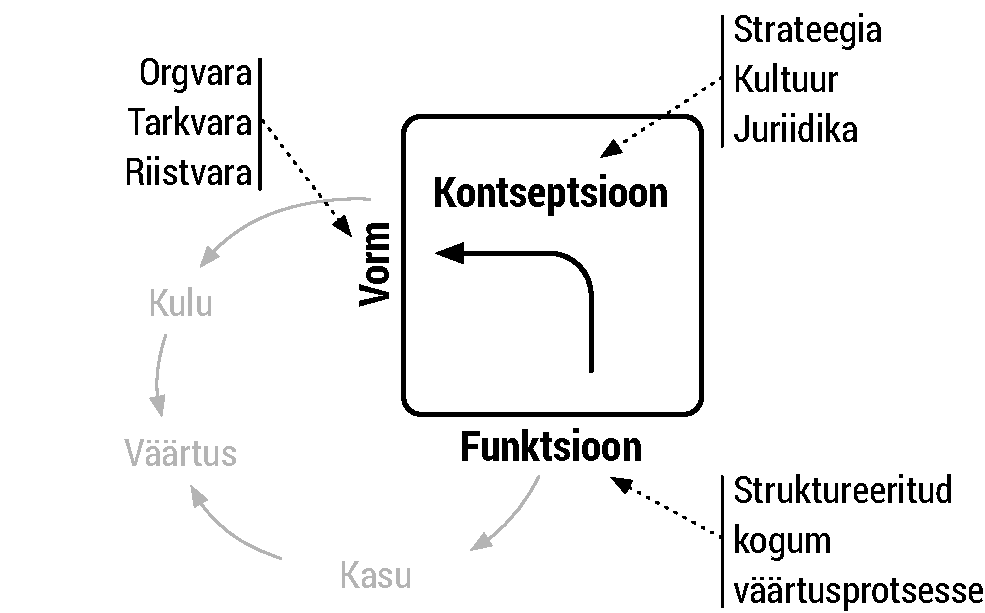
\includegraphics[width=.7\textwidth]{ffc_profit.pdf}
	\end{center}
\end{frame}

\begin{frame}[fragile]
	\frametitle{Arhitektuur ja äri}
			\begin{itemize}
				\item Arhitektuur määrab toote või teenuse \emph{võimekuse} kasumit teenida
				\item Sealhulgas
				\begin{itemize}
					\item Tootmiskulud. Kui kallist programmerijat teie arhitektuur eeldab?
					\item Halduskulud. Kas olemasolevad adminid tulevad toime?
					\item Väljumiskulud. Kui keeruline on teie tarkvarast loobuda?
				\end{itemize}
				\item Arhitekt peab ettevõtte ärimudelist väga hästi aru saama ja suutma tolle arusaamaga midagi ette võtta
			\end{itemize}
\end{frame}
\note{Oluline rõhk võimekusel. Mäletate: arhitektuur määrab vektorid, mille sisustab disain. Kui aga parameetrid on paigast ära, ei tule kasumist midagi. Ehk. Vale arhitektuur tähendab, et äri ei saa olla kasumlik, õige arhitektuur ei tähenda, et äri on kasumlik.}

%Arutelu koht
\begin{frame}[fragile]
  \frametitle{Arutelu koht}
		\begin{center}
			\textbf{Kuidas seletada kliendile, et ta saab sama raha eest täna vähem, kui eile?}
		\end{center}
\end{frame}

\section{Tarkvaratehnika}
\begin{frame}[fragile]
  \frametitle{Tarkvaratehnika definitisioon}
	\begin{center}
		\begin{quote}
			Tarkvaratehnika on süstemaatiline lähenemine tarkvara analüüsile, disainile, hindamisele, realiseerimisele, testimisele, haldamisele ja ümbertöötamisele, ehk, inseneriteaduse rakendamine tarkvarale.
		\end{quote}		
	\end{center}
	\cite{laplante}
\end{frame}
\note{Väga asjalik raamat, nii palju kui sirvida jõudsin. Annab kena ülevaate, mis üldse tarkvaratehnikas toimub}

\begin{frame}[fragile]
  \frametitle{Definitsiooni järelmid}
	\begin{itemize}
		\item Mainitud seitset eri distsipliini, realisatsioon on vaid üks neist
		\note{Siit peaks tulema vihje rõhuasetuste kohta: enamasti keskendutakse programmeerimisele\\}
		\item Ei ole viidet arendusprotsessile, kui sellisele
			\begin{itemize}
				\item Distsipliine saab kokku panna väga mitmel eri viisil, milline on parim?
				\item Igapäevases elus saab arendusprotsess disproportsionaalselt palju tähelepanu
				\note{Sest kvarteti liikmeid ümber paigutada on lihtne, mõistliku testimisraamistiku välja töötamine aga väga keeruline\\}
			\end{itemize}
		\item Kenasti on kaetud tarkvara elutsükkel, ümbertöötamine (ingl. \emph{reengineering}) on samuti osa protsessist ja oluline kuluallikas
	\end{itemize}
\end{frame}
\note{Programmeerijad on tarkvaratehnika kaaperdanud tõmmates tähelepanu endale ja jättes varju teised valdkonnad. Mis, muidugi, võtavad ära suurema osa ka nende päevast kuid siiski kutsutakse neid 'programmeerijateks'}

\begin{frame}[fragile]
  \frametitle{Tarkvaratehnika olulisus}
  Äristrateegia on otseselt seotud valitud viisiga tarkvara ehitada. Joel \citep{spolsky2004joel2} kirjeldab kenasti Amazon vs. Ben \& Jerry's dilemmat
  \begin{itemize}
  	\item Orgaaniline kasv vs. Ruttu Suureks lähenemine
	\item Head näited tarkvaratehniliste valikute osas
		  \begin{itemize}
		  	\item Kas probleemile lähenetakse raha või mõtlemisega?
			\item Kui oluline on toodetud koodi kvaliteet?
			\item Kas protsess toetab on kiiret rabelemist või jätkusuutlikku arengut?
		  \end{itemize}
	\item Õige vastus sõltub valitud strateegiast. Seega
  \end{itemize}
  \begin{center}
	  \textbf{Otsusta üheselt, kas oled Amazon või Ben \& Jerry's}
  \end{center}
\end{frame}
\note{Lugege Joeli, ta on hea. Suurem osa sisu veebis tasuta saadaval aga raamat on mugavam}
\note{Muidugi on toodud vastuolu vaid üks võimalikke, kuid illustreerib seoseid kenasti}

\begin{frame}[fragile]
  \frametitle{Tarkvaratehnika keerukus}
	Brooks ütleb oma essees \citep{brooks1975mythical}, et \emph{Tarkvara ehitamine on oma olemuselt keeruline}, see ei saa kunagi lihtne olema. 
  \begin{itemize}
	\item Läbi aja on üritatud hõbekuuli siiski leida
		  \begin{itemize}
		  	\item Nõuete kirjeldamine
			\item Mingi protsessi kasutamine
			\item Artefaktide tootmine
			\item "Tagasi loodusse" protsesse eitavad lähenemised
		  \end{itemize}
	\item Keskendu olulisele ja ära lase endale mao-õli müüa
	\note{Tuletage meelde tarkvaratehnika definitsiooni, katsuge igaühte neist võimalikult hästi teha ning siduge tükid kokku nii, nagu mõnus tundub\\}
  \end{itemize}
\end{frame}
\note{Ülejäänud Brooks on ka hea, "The mythical man-month" essee peaks olema kohustuslik igale programmeerijaid juhtivale inimesele}


%Arutelu koht
\begin{frame}[fragile]
  \frametitle{Arutelu koht}
		\begin{center}
			\textbf{Mis teeb programmeerimise keeruliseks?}
		\end{center}
\end{frame}

\begin{frame}[fragile]
  \frametitle{Tarkvaratehnika}
	\begin{itemize}
		\item Mõistliku koodi 12 reeglit \cite{spolsky2004joel}
	\end{itemize}
\end{frame}

\begin{frame}[fragile]
  \frametitle{Mõistliku koodi reeglid}
  Mõistliku koodi 12 reeglit \cite{spolsky2004joel}
\small  
	\begin{enumerate}
		\item Kas sa kasutad (mõistlikku) koodikontrolli?
		\item Kas ehitamine on tehtav ühe sammuga?
		\item Kas sa ehitad iga päev?
		\item Kas sul on probleemihoidla?
		\item Kas sa parandad enne uue koodi kirjutamist vead?
		\item Kas sul on kuskil olemas kehtiv projektiplaan?
		\item Kas sul on spetsifikatsioon?
		\item Kas programmeerijatel on rahu ja vaikust?
		\item Kas sa kasutad parimaid tööriistu, mida raha eest saab?
		\item Kas sul on testijad?
		\item Kas uued tulijad kirjutavad intervjuu ajal koodi?
		\item Kas sa teed kiireid kasutatavusteste?
	\end{enumerate}
\normalsize
\end{frame}


\begin{frame}[fragile]
  \frametitle{Tehniline võlg}
	Tehniline võlg tekib, kui mõistliku lahenduse asemel tehakse mittemõistlik. NB! Tegu on \emph{metafooriga} ja tal on piirid.
  \begin{itemize}
	\item Teda võib teatud piirini võrrelda rahalise kohustusega
	\item Ta tuleb investeerida viisil, mis katab hilisemad intressikulud
	\item Tehnilise võla põhjus peaks olema äriline, kuid võib olla ka tehniline 
	\item Vaid ITl on võimekus hallata tehnilise võla portfelli
	\item Tehnilise võla likvideerimisel on reeglina ärilised põhjused kuid võivad olla ka tehnilised
  \end{itemize}

\end{frame}

\begin{frame}[fragile]
  \frametitle{Tehnilise võla kvadrant}
  	\begin{center}
			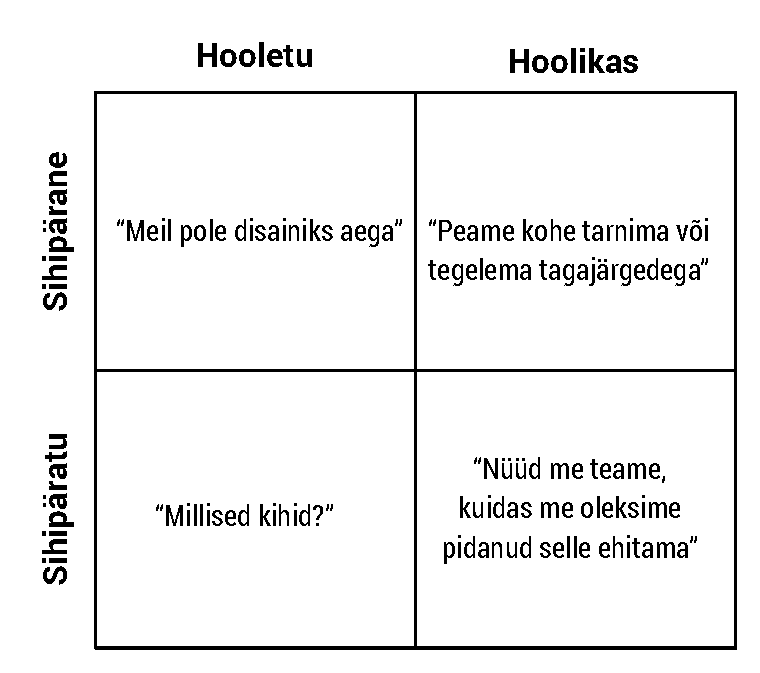
\includegraphics[width=.65\textwidth]{fowler.pdf}
	\end{center}
	\cite{fowlerdebt}
\end{frame}

%Arutelu koht
\begin{frame}[fragile]
  \frametitle{Arutelu koht}
		\begin{center}
			\textbf{Kuidas seletada tehnilist võlga juhtkonnale?}
		\end{center}
\end{frame}

\section{IT valitsemine}
\begin{frame}[fragile]
  \frametitle{IT valitsemine}
	\begin{itemize}
		\item Management vs. leadership. Manager is expendable, leader is not
		\item Mida me juhime, kui me juhime ITd? Inimesed, ressursid, protsessid
		\item Policy resistance olemus?
	\end{itemize}
\end{frame}

\begin{frame}[fragile]
  \frametitle{Inimesed}
	\begin{itemize}
		\item Inimesed käituvad viisil, mis maksimeerib nende huvisid. Kas need huvid on ettevõtte huvidega sobivad, on juhi mure
		\item Enne, kui inimesi valitsema/kontrollima hakata, küsi: kes läheb ära ja kes saab edukaks. \emph{Mitte} "kes jääb" 
	\end{itemize}
\end{frame}


%Arutelu koht
\begin{frame}[fragile]
  \frametitle{Arutelu koht}
		\begin{center}
			\textbf{Kuidas mõõta programmeerija tulemust?}
		\end{center}
\end{frame}

\begin{frame}[fragile]
  \frametitle{Ressursid}
	\begin{itemize}
		\item Kriitiline vahe riigi- ja erasektori vahel ressursijuhtimisel
		\item Ülesanne on alati maksimeerida bang per buck. Kõik muu on irrelevantne
		\item Seos tehnilise võlaga. Veendu, et tellija saab aru oma otsuste pikaajalisest rahalisest mõjust
		\item Strateegilises plaanis ei ole ressursijuhtimise protsessid kriitilised, osta HR paperwork ja finants väljast
	\end{itemize}
\end{frame}

\begin{frame}[fragile]
  \frametitle{Protsessid}
	\begin{itemize}
		\item Küberneetika kontrolli probleem. 
		\item Süsteemide loomulik inerts, eri tüüpi tasakaalud, beer game
		\item Jaapani mõtteviis (high velocity edge viited)
	\end{itemize}
\end{frame}


%Arutelu koht
\begin{frame}[fragile]
  \frametitle{Arutelu koht}
		\begin{center}
			\textbf{Kui palju peaks juhtkond teadma tehnilisest võlast?}
		\end{center}
\end{frame}

\begin{frame}[fragile]
  \frametitle{Arenduse pipeline}
	\begin{itemize}
		\item Miks see on oluline (kuigi läheb natuke taktikaliseks)
		\item Printsiibid: eelarve- ja otsusepõhine juhtimine. Nende tasakaalust. Suurte ja väikeste kivide probleem (seos tehnilise võlaga)
		\item Capacity, overflow ja pipeline otsused. Demand ületab alati supply. Järelikult jääb asju alati pipeline lõppu. On kriitiline, kuidas neid sealt välja võetakse
		\item Kuidas teha. Mõlemalt poolt mandaadiga juhid, regulaarne (veel parem: online), rolling, mitte spot
	\end{itemize}
\end{frame}

%Arutelu koht
\begin{frame}[fragile]
  \frametitle{Arutelu koht}
		\begin{center}
			\textbf{Mida teha, kui klient ei kuula?}
		\end{center}
\end{frame}


\section{Viited}

\begin{frame}[t,allowframebreaks,]
  	\bibliographystyle{plainnat}
	\bibliography{it_strateegia} 

\end{frame}

%\plain{Küsimusi?}
\begin{frame}[plain]
	\begin{center}Küsimusi?\end{center}
\end{frame}

\end{document}